% Beschreibung aller wichtigen Klassen und Schnitstellen inklusive der für ihr Verständnis wichtigen Methoden, Assoziationen und Attribute anhand eines/mehrerer Klassendiagramme. Eine GLiederung nach Paketen/Modulen kann oft sinnvoll sein.

\section{Datenbankzugriff}
Die zentrale Komponente unseres Systems ist die Datenbank. In sie fügt der Crawler neue Datensätze ein und aktualisiert vorhandene. Der Kategorisierer ist dafür zuständig, dass die gefundenen Accounts nach der DMOZ.org Datenbank in Kategorien unterteilt werden. Die GUI wiederum ist die Komponente die die Daten aus der Datenbank ausliest und visualisiert. Gegebenenfalls kann sie auch Einträge verändern beziehungsweise vervollständigen.//
Da alle unsere drei Systemkomponenten lesend, sowie schreibend auf die Datenbank zugreifen, haben wir uns entschlossen ein Paket für den Datenbankzugriff für alle Komponenten zur Verfügung stellen. Dieses sogenannte mysql-Package ist dann für den Auf- und Abbau der Verbindung zur Datenbank zuständig, sowie für das Schreiben und Lesen in beziehungsweise aus der Datenbank. Es stellt für jede der drei Komponenten ein eigenes Interface zur Verfügung, sodass jede Komponente nur die für sie erlaubten Änderungen an der Datenbank vornehmen kann.
Im folgenden ist der Aufbau des mysql-Packages zu sehen. Das darin eingeschlossene result-Package stellt Objekt und Methoden zu Verfügung um die Ergebnisse aus der Datenbank zu handeln.

\begin{figure}[p]
\includegraphics[width=\textwidth]{dia/uml_mysql-package}
\caption{UML-Klassendiagramm des mysql-Packages}
\end{figure}

\section{Crawler}

\begin{figure}[p]
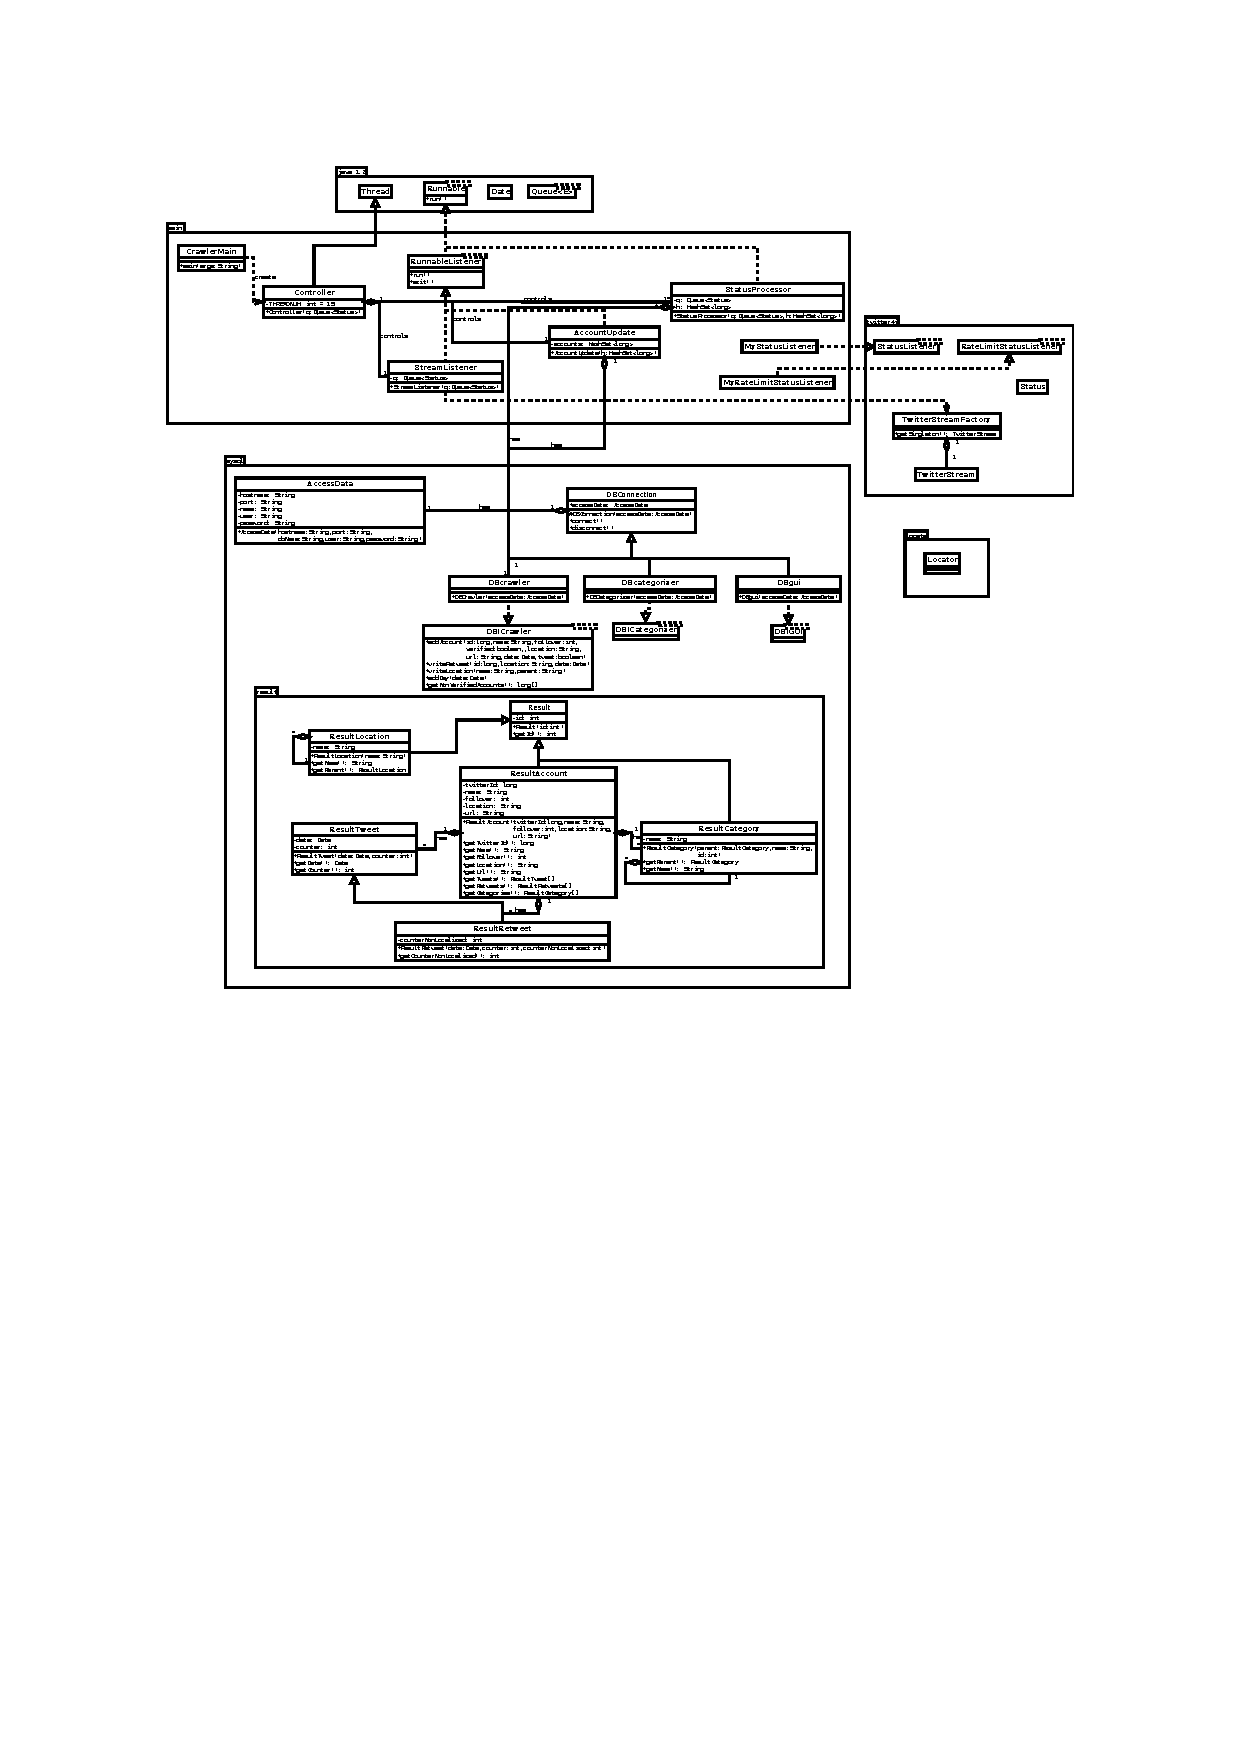
\includegraphics[width=\textwidth]{dia/uml_crawler}
\caption{UML-Klassendiagramm des Crawlers}
\end{figure}

\section{Kategorisierer}

\section{GUI}

